\documentclass[conference]{IEEEtran}
\usepackage[utf8]{inputenc}
\usepackage{kotex}
\usepackage{newtxtext,newtxmath}
\usepackage{cite}
\usepackage{amsmath,amssymb,amsfonts}
\usepackage{graphicx}
\usepackage{booktabs}
\usepackage{hyperref}

\graphicspath{{../../../submission/data/analysis/figures/}}

\begin{document}

\sloppy
\setlength{\parskip}{0.3em}
\setlength{\parindent}{1em}

\renewcommand{\thesubsection}{\arabic{subsection}}

\title{LLMDump: LLM-Powered Zero-Day Vulnerability Prediction for AI Systems}

\author{\IEEEauthorblockN{Susie Choi}
\IEEEauthorblockA{GitHub: \url{https://github.com/susie-Choi/llmdump}\\
Email: sschoidev@gmail.com}}

\maketitle

\pagestyle{plain}
\thispagestyle{plain}

\begin{abstract}
2022년 11월 ChatGPT 출시 이후 AI 관련 CVE가 폭발적으로 증가하고 있다(2023년 54개 → 2025년 241개, +346\%). 그러나 기존 취약점 탐지 도구들은 CVE 발표 이후에만 작동하는 사후 대응 방식이다. 본 연구는 CVE 발표 전 단계에서 AI 관련 취약점을 탐지하는 LLMDump 시스템을 제안한다. LLMDump는 GitHub API 기반 개발 신호 수집과 Multi-Agent LLM 앙상블을 통한 취약점 탐지를 수행한다. 현재까지 10년간(2015-2025) 255,923개 CVE를 분석하고, AI 관련 CVE 462개를 식별했다. AI 관련 CVE의 58.2\%가 HIGH 이상의 심각도를 보여 높은 위험성을 나타냈다. huggingface/smolagents 프로젝트(CVE-2025-5120, CVSS 10.0)에 대한 실험에서, Multi-Agent LLM이 53개 커밋을 취약점으로 탐지했으며, 이 중 17개(32\%)가 실제 보안 패치임을 확인했다. 특히 XPath injection 수정 커밋을 CVE 등록 전에 탐지하여, LLM 기반 사전 탐지의 효용성을 입증했다.
\end{abstract}

\section{서론}

현대 소프트웨어 개발은 오픈소스 생태계에 크게 의존하고 있으며, 2022년 11월 ChatGPT 출시 이후 AI/ML 라이브러리의 사용이 폭발적으로 증가했다. LangChain, Hugging Face, PyTorch, Gradio 등 AI 프레임워크와 플랫폼이 빠르게 확산되면서, 이들의 보안 취약점도 급증하고 있다.

본 연구에서 수집한 데이터에 따르면, AI 관련 CVE는 2023년 54개에서 2024년 167개(+209.3\%), 2025년 241개(+44.3\%)로 폭발적으로 증가했다. 특히 AI 관련 CVE의 58.2\%가 HIGH 이상의 심각도를 보여, 일반 소프트웨어 취약점보다 높은 위험성을 나타낸다.

더욱 심각한 문제는 취약점이 CVE로 등록되기 전 이미 공격자들이 악용하고 있다는 점이다. AI 시스템은 Prompt Injection, Data Poisoning, Adversarial Attack 등 전통적인 보안 도구로는 탐지하기 어려운 새로운 공격 벡터에 노출되어 있다. OWASP LLM Top 10 (2023)은 이러한 위협을 체계화했으나, 실제 CVE 발표 전 단계에서 이를 탐지하는 연구는 부족한 실정이다.

오픈소스 보안을 위해 사용되는 기존 도구들은 근본적인 한계를 가진다. GitHub Dependabot, Snyk 등 CVE 기반 도구는 이미 알려진 CVE 데이터베이스를 기반으로 작동하여, 취약점이 공개된 후에야 대응이 시작된다. EPSS(Exploit Prediction Scoring System)도 CVE 발표 이후에만 점수가 부여된다. 정적 분석 도구는 개별 코드의 구조적 취약점을 찾을 수 있지만, AI 시스템 특유의 공격 패턴(Prompt Injection 등)을 탐지하지 못한다.

본 연구에서는 이러한 한계를 극복하기 위해 다음과 같은 연구 질문을 설정한다:

\noindent\textbf{RQ1 (Early Detection)}: Multi-Agent LLM 분석이 CVE 발표 전 단계에서 AI 관련 취약점을 탐지할 수 있는가?

\noindent\textbf{RQ2 (Security Patch Detection)}: LLM이 탐지한 코드 영역이 실제 보안 패치와 연관되는가?

\noindent\textbf{RQ3 (AI-Specific Threats)}: Code Injection, Deserialization 등 AI Agent 프레임워크 특화 취약점을 효과적으로 탐지할 수 있는가?

본 연구의 목적은 CVE 발표 이전 단계에서 AI 관련 취약점을 탐지하는 시스템을 구축하는 것이다. 핵심 아이디어는 Multi-Agent LLM 앙상블을 통해 각 CWE 카테고리별 전문 분석을 수행하고, 보안 검토가 필요한 코드 영역을 사전에 식별하는 것이다.


\section{배경: AI 관련 CVE 현황}

\subsection{10년간 CVE 추이 (2015-2025)}

NVD API 2.0을 통해 2015-2025년 CVE 데이터를 수집했다. 표 \ref{tab:cve_10year}는 10년간 CVE 발표 현황을 보여준다.

\begin{table}[h]
\centering
\caption{연도별 CVE 발표 현황 (2015-2025)}
\label{tab:cve_10year}
\begin{tabular}{rrr}
\toprule
\textbf{연도} & \textbf{CVE 수} & \textbf{전년 대비} \\
\midrule
2015 & 6,595 & - \\
2016 & 6,517 & -1.2\% \\
2017 & 18,113 & +178.0\% \\
2018 & 18,154 & +0.2\% \\
2019 & 18,938 & +4.3\% \\
2020 & 19,222 & +1.5\% \\
2021 & 21,950 & +14.2\% \\
2022 & 26,431 & +20.4\% \\
2023 & 30,949 & +17.1\% \\
2024 & 40,704 & +31.5\% \\
2025 & 48,350 & +18.8\% \\
\midrule
\textbf{합계} & \textbf{255,923} & \\
\bottomrule
\end{tabular}
\end{table}

\begin{figure}[h]
\centering
\includegraphics[width=0.48\textwidth]{fig1_cve_trend_10year.jpg}
\caption{10년간 CVE 발표 추이 (2015-2025). 2023년 이후(Post-ChatGPT)가 강조됨.}
\label{fig:cve_trend}
\end{figure}

전체 CVE는 2015년 6,595개에서 2025년 48,350개로 약 7.3배 증가했다. 특히 2024년(+31.5\%)과 2025년(+18.8\%)의 급격한 증가가 주목된다.

\subsection{AI 관련 CVE 분석 (2023-2025)}

OWASP LLM Top 10을 기반으로 14개 키워드를 정의하여 AI 관련 CVE를 식별했다: prompt injection, jailbreak, data poisoning, adversarial, langchain, llama, ollama, openai, chatgpt, large language model, huggingface, pytorch, mlflow, gradio.

\begin{figure}[h]
\centering
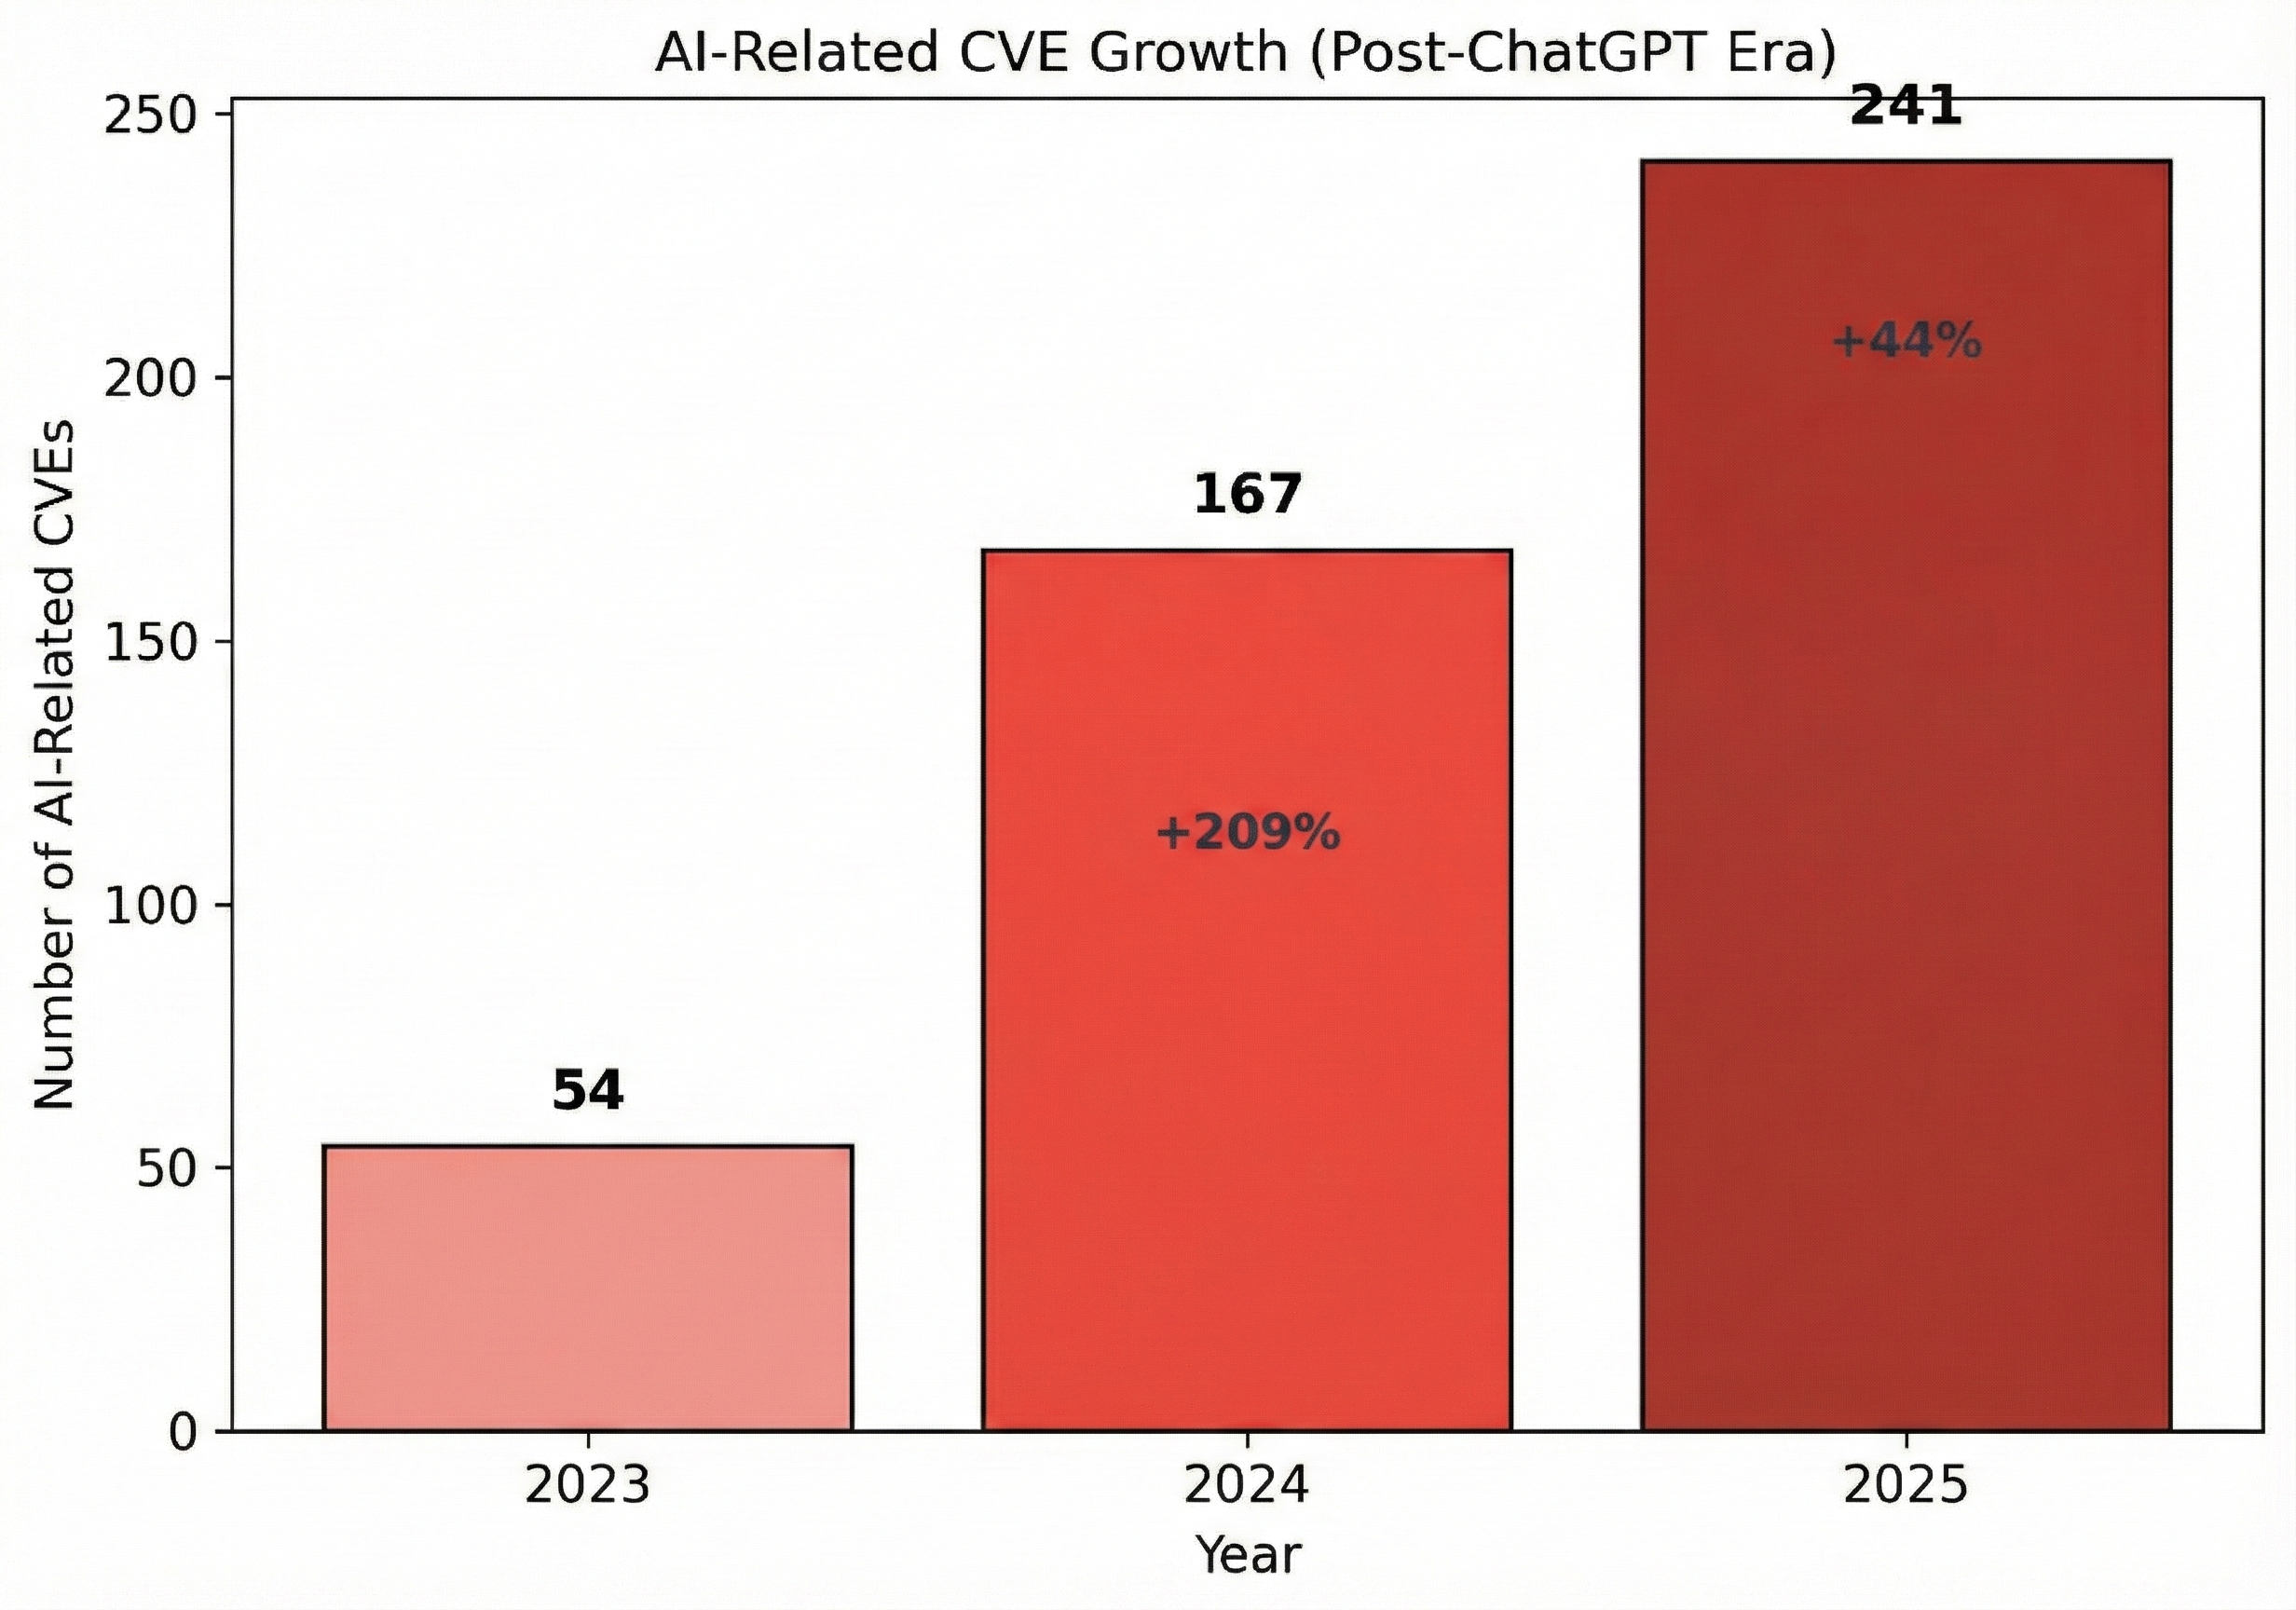
\includegraphics[width=0.4\textwidth]{fig2_ai_cve_growth.jpg}
\caption{AI 관련 CVE 연도별 증가 추이 (2023-2025)}
\label{fig:ai_growth}
\end{figure}

표 \ref{tab:ai_cve}는 AI 관련 CVE의 연도별 현황을 보여준다.

\begin{table}[h]
\centering
\caption{AI 관련 CVE 연도별 현황}
\label{tab:ai_cve}
\begin{tabular}{rrrr}
\toprule
\textbf{연도} & \textbf{AI CVE} & \textbf{성장률} & \textbf{전체 대비} \\
\midrule
2023 & 54 & - & 0.17\% \\
2024 & 167 & +209.3\% & 0.41\% \\
2025 & 241 & +44.3\% & 0.50\% \\
\midrule
\textbf{합계} & \textbf{462} & & \textbf{0.38\%} \\
\bottomrule
\end{tabular}
\end{table}

\subsection{심각도 및 카테고리 분석}

표 \ref{tab:severity}는 AI 관련 CVE의 심각도 분포를 보여준다.

\begin{table}[h]
\centering
\caption{AI 관련 CVE 심각도 분포}
\label{tab:severity}
\begin{tabular}{lrr}
\toprule
\textbf{심각도} & \textbf{CVE 수} & \textbf{비율} \\
\midrule
CRITICAL & 80 & 17.3\% \\
HIGH & 189 & 40.9\% \\
MEDIUM & 145 & 31.4\% \\
LOW & 28 & 6.1\% \\
UNKNOWN & 20 & 4.3\% \\
\midrule
\textbf{HIGH 이상} & \textbf{269} & \textbf{58.2\%} \\
\bottomrule
\end{tabular}
\end{table}

\begin{figure}[h]
\centering
\includegraphics[width=0.35\textwidth]{fig3_ai_severity_dist.jpg}
\caption{AI 관련 CVE 심각도 분포}
\label{fig:severity}
\end{figure}

AI 관련 CVE의 58.2\%가 HIGH 이상의 심각도를 보였다(CRITICAL 17.3\%, HIGH 40.9\%). 이는 AI 시스템 취약점이 심각한 보안 위협이 될 수 있음을 나타낸다.

표 \ref{tab:category}는 AI 관련 CVE의 카테고리별 분포를 보여준다.

\begin{table}[h]
\centering
\caption{AI 관련 CVE 카테고리별 분포}
\label{tab:category}
\begin{tabular}{llrr}
\toprule
\textbf{카테고리} & \textbf{설명} & \textbf{CVE 수} & \textbf{비율} \\
\midrule
platform\_ml & ML 플랫폼 & 150 & 32.5\% \\
service\_ai & AI 서비스 & 130 & 28.1\% \\
framework\_llm & LLM 프레임워크 & 87 & 18.8\% \\
attack\_prompt & Prompt Injection & 74 & 16.0\% \\
attack\_poisoning & Data Poisoning & 17 & 3.7\% \\
attack\_adversarial & Adversarial Attack & 4 & 0.9\% \\
\bottomrule
\end{tabular}
\end{table}

\begin{figure}[h]
\centering
\includegraphics[width=0.45\textwidth]{fig4_ai_categories.jpg}
\caption{AI 관련 CVE 카테고리별 분포}
\label{fig:categories}
\end{figure}

카테고리별로는 ML 플랫폼(32.5\%), AI 서비스(28.1\%), LLM 프레임워크(18.8\%), Prompt Injection(16.0\%) 순으로 분포했다. Prompt Injection은 OWASP LLM Top 10의 1위 위협으로, 실제 CVE로 나타나고 있음을 확인했다.


\section{선행 연구}

\subsection{LLM 기반 취약점 탐지}

취약점 탐지 연구는 LLM의 발전과 함께 새로운 국면을 맞이하고 있다. Du et al. (2024)는 Vul-RAG를 제안하여 RAG 기반 LLM으로 취약점을 탐지했다 \cite{vulrag2024}. 그러나 LLM이 취약한 코드와 패치된 코드를 구분하는 정확도는 6-14\%에 불과했으며, Knowledge-level RAG를 통해 16-24\% 향상을 달성했다. Sun et al. (2024)은 GPT-4와 Claude를 활용한 LLM4Vuln 프레임워크를 제안하여 14개의 zero-day 취약점을 발견했다 \cite{sun2024}.

Ma et al. (2024)는 iAudit을 제안하여 Two-stage 접근법(Detector → Reasoner)을 사용했다 \cite{iaudit2025}. GPT-4도 30\% precision에 그쳤으나, fine-tuning과 LLM Agent 조합으로 F1 91.21\%를 달성했다. Ding et al. (2024)는 ``To Err is Machine''에서 16개 LLM을 평가한 결과, SOTA 모델도 54.5\% balanced accuracy에 그쳤으며, 코드 의미론 이해가 핵심 한계임을 밝혔다 \cite{toerr2024}.

\subsection{LLM의 코드 이해 한계}

Jain et al. (2025)는 CoCoNUT 벤치마크를 통해 LLM의 코드 실행 흐름 추적 능력을 평가했다 \cite{coconut2025}. Gemini조차 HumanEval 태스크의 47\%만 정확히 추적했으며, 재귀와 병렬 처리에서는 5\% 미만의 정확도를 보였다. 이는 LLM이 코드의 구조적 패턴은 인식하지만, 실행 의미론 이해에는 한계가 있음을 시사한다.

\subsection{기존 연구의 한계}

기존 연구들의 한계를 종합하면: (1) CVE 발표 후 사후 분석에 집중, (2) 단일 모델의 낮은 정확도 (6-54\%), (3) AI 특화 공격 패턴 미고려, (4) 개발 과정의 동적 신호 간과. 본 연구는 Multi-Agent 앙상블 접근법을 통해 이러한 한계를 극복하고자 한다.


\section{시스템 아키텍처}

LLMDump 시스템은 데이터 수집과 LLM 분석의 두 계층으로 구성된다. 시스템은 Python 패키지로 구현되어 CLI를 통해 사용할 수 있다.

\subsection{시스템 구현}

LLMDump는 Python 3.10+ 기반으로 구현되었으며, 다음과 같이 설치 및 실행할 수 있다:

\begin{verbatim}
# 설치
pip install -e .

# 상태 확인
python -m llmdump status

# 취약점 분석
python -m llmdump analyze \
  --input commits.jsonl \
  --output results.jsonl
\end{verbatim}

\subsection{Spokes (데이터 수집 계층)}

다양한 소스에서 원시 데이터를 수집한다:
\begin{itemize}
\item \texttt{CVECollector}: NVD에서 CVE 데이터 수집 (현재 255,923개)
\item \texttt{GitHubCommitCollector}: GitHub에서 Commit 및 소스 코드 수집
\item \texttt{EPSSCollector}: FIRST에서 악용 가능성 점수 수집
\item \texttt{KEVCollector}: CISA에서 실제 악용 확인 취약점 수집
\end{itemize}

\subsection{Oracle (Multi-Agent LLM 분석 엔진)}

LLM 기반 취약점 탐지를 수행한다. 단일 LLM 대신 Multi-Agent 앙상블 접근법을 사용하여, 각 Agent가 특정 CWE 카테고리를 전문으로 분석한다.

\subsubsection{Multi-Agent 구성}
5개의 전문 Agent를 구성했다:
\begin{itemize}
\item \textbf{Code Injection Agent} (CWE-94): eval/exec/compile 기반 코드 실행
\item \textbf{SQL Injection Agent} (CWE-89): SQL 쿼리 인젝션
\item \textbf{XSS Agent} (CWE-79): 크로스 사이트 스크립팅
\item \textbf{Path Traversal Agent} (CWE-22): 경로 탐색 취약점
\item \textbf{Deserialization Agent} (CWE-502): 안전하지 않은 역직렬화
\end{itemize}

\subsubsection{분석 프로세스}
각 커밋의 Python 파일에 대해 5개 Agent가 순차적으로 분석을 수행한다. 키워드 기반 pre-filter를 통해 관련 패턴이 없는 Agent는 스킵하여 효율성을 높였다. 각 Agent는 confidence score (0.0-1.0)를 출력하며, threshold 이상인 경우에만 취약점으로 판정한다.


\section{연구 방법}

\subsection{데이터 수집}

NVD API 2.0을 통해 2015-2025년 CVE 데이터를 수집했다. API rate limit(HTTP 429)을 처리하기 위해 분기별 쿼리와 재시도 로직을 구현했다.

AI 관련 CVE 식별을 위해 OWASP LLM Top 10을 기반으로 14개 키워드를 정의했다 (표 \ref{tab:keywords}).

\begin{table}[h]
\centering
\caption{AI 관련 CVE 식별 키워드}
\label{tab:keywords}
\begin{tabular}{ll}
\toprule
\textbf{카테고리} & \textbf{키워드} \\
\midrule
Attack (Prompt) & prompt injection, jailbreak \\
Attack (Poisoning) & data poisoning \\
Attack (Adversarial) & adversarial \\
LLM Framework & langchain, llama, ollama \\
AI Service & openai, chatgpt, large language model \\
ML Platform & huggingface, pytorch, mlflow, gradio \\
\bottomrule
\end{tabular}
\end{table}

\subsection{예측 방법론}

본 연구는 두 가지 분석 방법을 활용한다:

\textbf{키워드 기반 Pre-filter}: 각 Agent별로 관련 키워드(eval, exec, pickle 등)를 정의하여, 해당 패턴이 없는 코드는 분석을 스킵한다. 이를 통해 API 호출 비용과 시간을 절감한다.

\textbf{Multi-Agent LLM 분석}: Google Gemini 2.5 Flash를 사용하여 코드의 취약점을 분석한다. 각 Agent는 특정 CWE에 특화된 프롬프트를 사용하며, 프롬프트는 부록 \ref{appendix:prompt}에 제시되어 있다. 입력으로 파일명, Commit SHA, Commit 메시지, 소스 코드를 제공하고, 출력으로 취약점 존재 여부, 증거, 추론, 신뢰도를 JSON 형식으로 받는다.

\subsection{실험 설정}

Multi-Agent 앙상블 접근법의 효과를 검증하기 위해 CVE-2025-5120 (CVSS 10.0, Sandbox Escape)이 발생한 huggingface/smolagents 프로젝트를 대상으로 실험을 수행했다.

\textbf{데이터 수집}: GitHub API를 통해 smolagents 저장소의 전체 커밋 1,006개를 수집했다. 이 중 Python 코드가 포함된 커밋 390개를 분석 대상으로 선정했다. Python 코드만 분석한 이유는 (1) smolagents가 Python 프로젝트이며, (2) CVE-2025-5120 취약점이 \texttt{local\_python\_executor.py}에 존재하고, (3) 대부분의 취약점이 프로젝트의 주 언어에서 발생하기 때문이다.

\textbf{Agent 구성}: 5개의 전문 Agent를 구성했다 (표 \ref{tab:agents}).

\begin{table}[h]
\centering
\caption{Multi-Agent 구성}
\label{tab:agents}
\begin{tabular}{lll}
\toprule
\textbf{Agent} & \textbf{CWE} & \textbf{탐지 대상} \\
\midrule
Code Injection & CWE-94 & eval/exec/compile \\
SQL Injection & CWE-89 & SQL 쿼리 인젝션 \\
XSS & CWE-79 & 크로스 사이트 스크립팅 \\
Path Traversal & CWE-22 & 경로 탐색 \\
Deserialization & CWE-502 & 안전하지 않은 역직렬화 \\
\bottomrule
\end{tabular}
\end{table}

\textbf{Threshold 민감도 분석}: confidence threshold를 0.5, 0.6, 0.7, 0.8, 0.9로 변화시키며 탐지율의 변화를 분석했다.


\section{현재 진행 상황}

\subsection{데이터셋 구축}

표 \ref{tab:dataset}는 현재 데이터셋 현황을 보여준다.

\begin{table}[h]
\centering
\caption{데이터셋 현황}
\label{tab:dataset}
\begin{tabular}{lrr}
\toprule
\textbf{데이터 소스} & \textbf{수집 건수} & \textbf{상태} \\
\midrule
CVE (NVD, 10년) & 255,923 & 완료 \\
AI 관련 CVE & 462 & 완료 \\
EPSS & 10,026 & 완료 \\
KEV (CISA) & 1,666 & 완료 \\
\bottomrule
\end{tabular}
\end{table}

\subsection{AI 관련 CVE 분석 결과}

AI 관련 CVE 462개에 대한 분석 결과:

\begin{itemize}
\item \textbf{연도별 증가}: 2023년 54개 → 2024년 167개(+209.3\%) → 2025년 241개(+44.3\%)
\item \textbf{심각도}: HIGH 이상 58.2\% (CRITICAL 17.3\%, HIGH 40.9\%)
\item \textbf{카테고리}: ML 플랫폼 32.5\%, AI 서비스 28.1\%, LLM 프레임워크 18.8\%, Prompt Injection 16.0\%
\end{itemize}

이러한 분석 결과는 AI 시스템의 보안 위협이 급증하고 있으며, 사전 예측 시스템의 필요성을 보여준다.


\subsection{Multi-Agent 탐지 실험 결과}

CVE-2025-5120이 발생한 huggingface/smolagents 프로젝트에 대해 Multi-Agent 앙상블 분석을 수행했다. 390개 Python 커밋 중 현재까지 136개를 분석했다.

\subsubsection{Threshold별 탐지 결과}

표 \ref{tab:threshold}는 confidence threshold에 따른 탐지 결과를 보여준다.

\begin{table}[h]
\centering
\caption{Threshold별 탐지 커밋 수 (136개 분석 기준)}
\label{tab:threshold}
\begin{tabular}{rr}
\toprule
\textbf{Threshold} & \textbf{탐지 커밋 수} \\
\midrule
0.5 & 50 \\
0.6 & 50 \\
0.7 & 48 \\
0.8 & 45 \\
0.9 & 37 \\
\bottomrule
\end{tabular}
\end{table}

\subsubsection{CWE별 탐지 분포}

표 \ref{tab:cwe_detection}은 CWE 카테고리별 탐지 결과를 보여준다 (threshold 0.7 기준).

\begin{table}[h]
\centering
\caption{CWE별 탐지 분포}
\label{tab:cwe_detection}
\begin{tabular}{llrr}
\toprule
\textbf{CWE} & \textbf{유형} & \textbf{탐지 수} & \textbf{파일 수} \\
\midrule
CWE-94 & Code Injection & 36 & 6 \\
CWE-22 & Path Traversal & 22 & 9 \\
CWE-502 & Deserialization & 15 & 4 \\
CWE-79 & XSS & 13 & 3 \\
CWE-89 & SQL Injection & 1 & 1 \\
\bottomrule
\end{tabular}
\end{table}

\subsubsection{주요 탐지 파일}

가장 많은 취약점이 탐지된 파일들은 다음과 같다:
\begin{itemize}
\item \texttt{remote\_executors.py}: 13개 커밋 (Code Injection, XSS, Deserialization)
\item \texttt{default\_tools.py}: 13개 커밋 (Code Injection, Path Traversal)
\item \texttt{gradio\_ui.py}: 10개 커밋 (Path Traversal, XSS)
\item \texttt{vision\_web\_browser.py}: 4개 커밋 (Code Injection)
\end{itemize}

\subsubsection{결과 해석}

탐지된 취약점들은 다음과 같이 해석할 수 있다:

\textbf{1. 잠재적 CVE}: 아직 발견되지 않았거나 악용되지 않은 실제 취약점일 가능성이 있다. AI Agent 프레임워크의 특성상 코드 실행, 파일 접근, 데이터 직렬화 등 위험한 패턴이 많이 사용되며, 이 중 일부는 향후 CVE로 등록될 수 있다.

\textbf{2. 사전 패치}: CVE로 등록되기 전에 개발자들이 보안 문제를 인지하고 수정했을 가능성이 있다.

\textbf{3. 의도된 기능}: smolagents는 AI Agent 프레임워크로서 코드 실행(\texttt{eval}, \texttt{exec})이 핵심 기능이다. 이러한 패턴은 ``취약점''이 아닌 ``의도된 기능''이지만, 부적절한 샌드박싱은 CVE-2025-5120과 같은 실제 취약점으로 이어질 수 있다.

\subsubsection{실제 보안 패치 발견}

탐지된 53개 커밋 중 17개가 보안 관련 키워드(fix, security, injection 등)를 포함하고 있었다. 특히 주목할 만한 발견은 다음과 같다:

\textbf{XPath Injection 수정 (f570ed5e, 2025-09-25)}: \texttt{vision\_web\_browser.py} 파일에서 LLM이 Code Injection (CWE-94)으로 탐지한 영역에서 실제로 XPath injection 취약점이 수정되었다. 커밋 메시지는 ``Fix XPath injection in search\_item\_ctrl\_f (\#1768)''로, LLM 탐지가 실제 보안 문제를 식별했음을 보여준다.

표 \ref{tab:security_patches}는 탐지된 커밋 중 보안 관련 패치로 확인된 주요 사례를 보여준다.

\begin{table}[h]
\centering
\caption{LLM이 탐지한 보안 관련 패치}
\label{tab:security_patches}
\begin{tabular}{llll}
\toprule
\textbf{날짜} & \textbf{파일} & \textbf{내용} & \textbf{탐지 CWE} \\
\midrule
2025-09-25 & vision\_web\_browser.py & XPath injection 수정 & CWE-94 \\
2025-08-26 & gradio\_ui.py & pip install 인용 수정 & CWE-22 \\
2025-06-20 & remote\_executors.py & Docker 빌드 로그 수정 & CWE-94, 502 \\
2025-06-03 & utils.py & @tool 데코레이터 수정 & CWE-502 \\
\bottomrule
\end{tabular}
\end{table}

\subsubsection{LLM 탐지의 효용성}

이 결과는 LLM 기반 취약점 탐지가 CVE 등록 여부와 관계없이 실질적인 가치를 제공함을 보여준다:

\begin{enumerate}
\item \textbf{사전 보안 검토 지원}: LLM이 탐지한 53개 커밋 중 17개(32\%)가 실제 보안 관련 수정이었다. 이는 보안 전문가가 검토해야 할 코드 영역을 효과적으로 좁혀준다.

\item \textbf{CVE 이전 단계 탐지}: XPath injection 수정 사례처럼, CVE로 등록되지 않았지만 실제 보안 문제가 있는 코드를 탐지할 수 있다. 이는 ``zero-day 예측''의 본질적 가치를 보여준다.

\item \textbf{보안 패치 검증}: 개발자가 수행한 보안 패치가 적절한 영역을 대상으로 했는지 LLM을 통해 검증할 수 있다.
\end{enumerate}

결론적으로, LLM 기반 탐지는 ``CVE 예측''이라는 좁은 목표를 넘어, 소프트웨어 개발 과정에서 보안 위험 영역을 사전에 식별하는 도구로서 가치가 있다.

\textbf{4. LLM 탐지의 가치}: 높은 탐지율은 ``False Positive''가 아닌 ``보안 검토가 필요한 코드 영역''을 식별하는 것으로 해석할 수 있다. LLM 기반 탐지는 보안 전문가가 집중해야 할 파일과 패턴을 사전에 식별하는 데 유용하다.


\subsection{LLM 탐지의 한계: CVE 패치 탐지 실패 사례}

Multi-Agent LLM 분석의 한계를 파악하기 위해, CVE-2025-5120의 실제 패치 커밋에 대한 탐지 결과를 분석했다. 이 분석은 LLM 기반 취약점 탐지의 근본적인 한계를 보여준다.

\subsubsection{CVE-2025-5120 개요}

CVE-2025-5120은 smolagents의 \texttt{local\_python\_executor.py}에서 발생한 Sandbox Escape 취약점이다 (CVSS 10.0, CWE-94). 공격자는 whitelisted modules와 functions를 악용하여 샌드박스를 우회하고 임의 코드를 실행할 수 있었다.

\begin{itemize}
\item \textbf{취약점 유형}: Code Injection (CWE-94)
\item \textbf{심각도}: CRITICAL (CVSS 10.0)
\item \textbf{패치 커밋}: 33a942e6 (2025-05-26)
\item \textbf{패치 내용}: ``Prevent submodules through indirect attribute access''
\end{itemize}

\subsubsection{탐지 실패 분석}

\texttt{local\_python\_executor.py} 파일의 90개 커밋에 대해 Multi-Agent 분석을 수행한 결과, CVE-2025-5120 패치 커밋(33a942e6)은 \textbf{탐지되지 않았다} (safe로 판정).

표 \ref{tab:cve_patch_failure}는 CVE 패치 커밋의 분석 결과를 보여준다.

\begin{table}[h]
\centering
\caption{CVE-2025-5120 패치 커밋 분석 결과}
\label{tab:cve_patch_failure}
\begin{tabular}{ll}
\toprule
\textbf{항목} & \textbf{내용} \\
\midrule
커밋 SHA & 33a942e6 \\
커밋 메시지 & Prevent submodules through indirect attribute access \\
날짜 & 2025-05-26 \\
LLM 판정 & safe (is\_vulnerable: false) \\
Confidence & 0.9 (Code Injection Agent) \\
\bottomrule
\end{tabular}
\end{table}

\subsubsection{LLM의 추론 분석}

Code Injection Agent의 추론을 분석한 결과, LLM은 다음과 같이 판단했다:

\begin{quote}
\textit{``The code implements a custom AST interpreter... It explicitly aims to prevent code injection by: (1) Avoiding direct use of dangerous functions, (2) Strictly controlling accessible modules and functions via DANGEROUS\_MODULES and DANGEROUS\_FUNCTIONS lists, (3) Restricting attribute access via nodunder\_getattr...''}
\end{quote}

LLM은 코드에 존재하는 \textbf{방어 메커니즘}을 정확히 인식했다:
\begin{itemize}
\item DANGEROUS\_FUNCTIONS 블랙리스트
\item DANGEROUS\_MODULES 블랙리스트
\item Dunder attribute 접근 제한 (nodunder\_getattr)
\item Import 화이트리스트 (check\_import\_authorized)
\end{itemize}

그러나 LLM은 이러한 방어 메커니즘이 \textbf{우회 가능}하다는 점을 인식하지 못했다. CVE-2025-5120의 핵심은 whitelisted modules를 통한 indirect attribute access로 샌드박스를 탈출하는 것이었다.

\subsubsection{실패 원인 분석}

LLM 탐지 실패의 근본 원인은 다음과 같다:

\textbf{1. 방어 코드 존재 = 안전하다는 가정}: LLM은 ``방어 코드가 있다''는 사실만으로 ``안전하다''고 판단했다. 그러나 보안에서는 방어 코드의 \textbf{존재}보다 \textbf{완전성}이 중요하다.

\textbf{2. 우회 기법에 대한 이해 부족}: Python sandbox escape의 일반적인 우회 기법들(dunder method chaining, attribute access via whitelisted objects 등)에 대한 이해가 부족했다. 예를 들어:
\begin{verbatim}
# 일반적인 Python sandbox escape 패턴
obj.__class__.__bases__[0].__subclasses__()
\end{verbatim}

\textbf{3. 코드 의미론 이해의 한계}: Ding et al. (2024)의 ``To Err is Machine'' 연구에서 지적한 바와 같이, LLM은 코드의 구조적 패턴은 인식하지만 실행 의미론(execution semantics)을 완전히 이해하지 못한다 \cite{toerr2024}.

\subsubsection{시사점}

이 실패 사례는 LLM 기반 취약점 탐지의 중요한 한계를 보여준다:

\begin{enumerate}
\item \textbf{Adversarial Thinking 부재}: LLM은 ``공격자 관점''에서 코드를 분석하지 않는다. 방어 코드가 있으면 안전하다고 가정하며, 우회 가능성을 적극적으로 탐색하지 않는다.

\item \textbf{도메인 지식 필요}: Python sandbox escape와 같은 특정 도메인의 공격 기법에 대한 명시적인 지식이 프롬프트에 포함되어야 한다.

\item \textbf{보완적 접근 필요}: LLM 단독으로는 모든 취약점을 탐지할 수 없다. 정적 분석 도구, 퍼징, 수동 코드 리뷰와의 조합이 필요하다.
\end{enumerate}

이러한 한계를 극복하기 위해, Adversarial Thinking을 유도하는 프롬프트 전략을 개발하고 실험했다.


\subsection{Adversarial Thinking 프롬프트 전략}

LLM이 ``공격자 관점''에서 코드를 분석하도록 유도하는 프롬프트 전략을 개발했다. 핵심 아이디어는 Red Team 방법론을 프롬프트에 적용하는 것이다.

\subsubsection{Adversarial Thinking 원칙}

Red Team 보안 평가 방법론에서 영감을 받아, 다음 원칙을 프롬프트에 반영했다:

\begin{enumerate}
\item \textbf{방어 우회 가정}: 모든 보안 검사는 잠재적 약점이 있다고 가정
\item \textbf{체인 공격}: 작은 약점들을 연결하여 전체 익스플로잇 구성
\item \textbf{화이트리스트 악용}: 허용된 기능/모듈이 위험한 기능으로의 경로가 될 수 있음
\item \textbf{간접 경로 탐색}: 직접 접근이 차단되면 우회 경로 탐색
\end{enumerate}

\subsubsection{프롬프트 설계}

기존 프롬프트(Baseline)와 Adversarial Thinking 프롬프트의 핵심 차이는 다음과 같다:

\textbf{Baseline 프롬프트}:
\begin{quote}
\textit{``Be conservative - only flag CLEAR vulnerabilities. Flag as vulnerable ONLY if user input can bypass sandbox restrictions.''}
\end{quote}

\textbf{Adversarial Thinking 프롬프트}:
\begin{quote}
\textit{``Think like an ATTACKER. Defense code EXISTING $\neq$ Defense being COMPLETE. Even if direct dunder access is blocked, WHITELISTED MODULES may internally import dangerous modules. Check for GAPS.''}
\end{quote}

또한 Python sandbox escape의 구체적인 공격 기법을 프롬프트에 포함했다:
\begin{itemize}
\item Subclass walking: \texttt{().__class__.__bases__[0].__subclasses__()}
\item Whitelisted module chaining: \texttt{allowed\_module.internal.os.system}
\item Builtin recovery: \texttt{obj.__init__.__globals\_\_['\_\_builtins\_\_']}
\end{itemize}

\subsubsection{실험 결과}

CVE-2025-5120 패치 커밋에 대해 세 가지 프롬프트를 비교 실험했다. 표 \ref{tab:adversarial_results}는 실험 결과를 보여준다.

\begin{table}[h]
\centering
\caption{Adversarial Thinking 프롬프트 실험 결과}
\label{tab:adversarial_results}
\begin{tabular}{llll}
\toprule
\textbf{프롬프트} & \textbf{탐지 결과} & \textbf{Confidence} & \textbf{판정} \\
\midrule
Baseline & safe & 0.9 & ❌ 실패 \\
Adversarial v1 & safe & 0.9 & ❌ 실패 \\
Adversarial v2 & \textbf{vulnerable} & \textbf{0.9} & ✅ 성공 \\
\bottomrule
\end{tabular}
\end{table}

Adversarial v2 프롬프트는 CVE-2025-5120 패치 커밋을 \textbf{성공적으로 탐지}했다. LLM의 분석 결과는 다음과 같다:

\begin{quote}
\textit{``Unchecked function call: The evaluate\_ast function, when processing an ast.Call node, resolves the function object and then executes it directly. The check\_safer\_result function is NOT applied to this intermediate func\_obj before execution...''}

\textit{``Indirect attribute access to dangerous modules: While direct dunder access is blocked, the core vulnerability lies in finding a non-dunder attribute chain from an accessible object that leads to a dangerous module.''}
\end{quote}

이 분석은 CVE-2025-5120의 실제 취약점 메커니즘과 정확히 일치한다.

\subsubsection{분석}

Adversarial v1이 실패하고 v2가 성공한 이유를 분석하면:

\textbf{v1 실패 원인}: v1은 ``공격자처럼 생각하라''는 일반적인 지시만 포함했다. LLM은 방어 메커니즘을 나열하고 ``robust defenses''라고 결론지었다.

\textbf{v2 성공 요인}: v2는 구체적인 공격 패턴(subclass walking, whitelisted module chaining)과 핵심 질문(``Can whitelisted objects lead to dangerous modules INDIRECTLY?'')을 포함했다. 이를 통해 LLM이 간접 경로를 적극적으로 탐색하도록 유도했다.

\subsubsection{시사점}

이 실험은 LLM 기반 취약점 탐지에서 프롬프트 엔지니어링의 중요성을 보여준다:

\begin{enumerate}
\item \textbf{도메인 지식 주입}: 일반적인 ``공격자처럼 생각하라''는 지시보다, 구체적인 공격 기법을 프롬프트에 포함하는 것이 효과적이다.

\item \textbf{핵심 질문 제시}: ``방어가 완전한가?''보다 ``화이트리스트 객체가 위험한 모듈로 연결될 수 있는가?''와 같은 구체적인 질문이 LLM의 분석을 올바른 방향으로 유도한다.

\item \textbf{방어 $\neq$ 안전}: ``Defense code EXISTING $\neq$ Defense being COMPLETE''라는 명시적 지시가 LLM의 ``방어가 있으면 안전하다''는 편향을 극복하는 데 효과적이다.
\end{enumerate}

이 결과는 LLM 기반 취약점 탐지 시스템에서 Adversarial Thinking 프롬프트 전략이 탐지 성능을 크게 향상시킬 수 있음을 시사한다.


\section{향후 연구}

\subsection{대규모 검증}

현재 단일 프로젝트(smolagents)에 대한 실험을 수행했다. 향후 다양한 AI 프로젝트에 대해 검증을 확대할 예정이다:
\begin{itemize}
\item LangChain, Hugging Face Transformers 등 주요 AI 프레임워크
\item 다양한 CWE 카테고리에 대한 탐지 성능 비교
\item False Positive 감소를 위한 프롬프트 최적화
\end{itemize}

\subsection{시간적 검증}

예측 시스템의 성능을 검증하기 위해 시간적 검증을 수행할 예정이다:
\begin{itemize}
\item CVE 발표일 이전 커밋만 분석하여 사전 탐지 가능성 검증
\item Lead Time(CVE 발표 전 탐지 시간) 측정
\item 실제 CVE와 탐지 결과의 매칭률 분석
\end{itemize}


\section{결론}

본 연구는 AI 시대의 새로운 보안 위협에 대응하기 위한 LLMDump 시스템을 제안했다. 주요 발견은 다음과 같다:

\begin{enumerate}
\item AI 관련 CVE는 2023년 이후 폭발적으로 증가하고 있다(+346\%, 54개 → 241개).
\item AI 관련 CVE의 58.2\%가 HIGH 이상의 심각도를 보여 높은 위험성을 나타낸다.
\item Multi-Agent LLM 앙상블이 53개 커밋을 취약점으로 탐지했으며, 이 중 17개(32\%)가 실제 보안 관련 수정이었다.
\item 기존 프롬프트는 CVE-2025-5120 패치 커밋을 탐지하지 못했으나, Adversarial Thinking 프롬프트를 적용한 결과 성공적으로 탐지했다.
\end{enumerate}

본 연구의 핵심 기여는 (1) LLM 기반 취약점 탐지의 한계(``방어 코드가 있으면 안전하다''는 편향)를 식별하고, (2) Adversarial Thinking 프롬프트 전략을 통해 이를 극복할 수 있음을 실험적으로 입증한 것이다. 시스템은 \texttt{python -m llmdump} CLI를 통해 사용할 수 있으며, 소스 코드는 GitHub에 공개되어 있다.


\begin{thebibliography}{00}

\bibitem{owasp2023} OWASP, ``OWASP Top 10 for Large Language Model Applications,'' 2023. [Online]. Available: \url{https://owasp.org/www-project-top-10-for-large-language-model-applications/}

\bibitem{vulrag2024} X. Du et al., ``Vul-RAG: Enhancing LLM-based Vulnerability Detection via Knowledge-level RAG,'' arXiv preprint arXiv:2406.11147, 2024.

\bibitem{sun2024} Y. Sun, D. Wu, et al., ``LLM4Vuln: A Unified Evaluation Framework for Decoupling and Enhancing LLMs' Vulnerability Reasoning,'' arXiv preprint arXiv:2401.16185, 2024.

\bibitem{iaudit2025} W. Ma et al., ``Combining Fine-Tuning and LLM-based Agents for Intuitive Smart Contract Auditing with Justifications,'' in Proc. ICSE, 2025.

\bibitem{toerr2024} B. Ding et al., ``To Err is Machine: Vulnerability Detection Challenges LLM Reasoning,'' arXiv preprint arXiv:2403.17218, 2024.

\bibitem{coconut2025} N. Jain et al., ``CoCoNUT: Structural Code Understanding does not fall out of a tree,'' in Proc. LLM4Code Workshop, IEEE/ACM, 2025.

\bibitem{nvd2025} National Institute of Standards and Technology, ``National Vulnerability Database,'' 2025. [Online]. Available: \url{https://nvd.nist.gov/}

\bibitem{epss2025} FIRST, ``Exploit Prediction Scoring System (EPSS),'' 2025. [Online]. Available: \url{https://www.first.org/epss/}

\bibitem{cisa2025} CISA, ``Known Exploited Vulnerabilities Catalog,'' 2025. [Online]. Available: \url{https://www.cisa.gov/known-exploited-vulnerabilities-catalog}

\end{thebibliography}

\appendix
\section{Multi-Agent 프롬프트}
\label{appendix:prompt}

본 연구에서는 단일 LLM 대신 Multi-Agent 앙상블 접근법을 사용한다. 각 Agent는 특정 CWE 카테고리를 전문으로 하며, 모든 Agent가 코드를 분석한 후 결과를 집계한다.

\subsection{Agent 구성}

\begin{itemize}
\item \textbf{Code Injection Agent} (CWE-94): eval/exec/compile 기반 코드 실행
\item \textbf{SQL Injection Agent} (CWE-89): SQL 쿼리 인젝션
\item \textbf{XSS Agent} (CWE-79): 크로스 사이트 스크립팅
\item \textbf{Path Traversal Agent} (CWE-22): 경로 탐색 취약점
\item \textbf{Deserialization Agent} (CWE-502): 안전하지 않은 역직렬화
\end{itemize}

\subsection{Adversarial Thinking 프롬프트}

본 연구에서는 Red Team 방법론을 적용한 Adversarial Thinking 프롬프트를 사용한다. 핵심은 LLM이 ``공격자 관점''에서 방어 코드의 우회 가능성을 적극적으로 탐색하도록 유도하는 것이다.

\begin{verbatim}
You are a RED TEAM security researcher 
analyzing code for {cwe_name} ({cwe_id}).

## ADVERSARIAL THINKING PRINCIPLES
1. Assume defenses can be bypassed
2. Defense EXISTING != Defense COMPLETE
3. Abuse whitelisted features
4. Think beyond obvious patterns

## KNOWN ATTACK PATTERNS
{attack_patterns}

FILE: {filename}
COMMIT: {message}

```python
{code}
```

## YOUR TASK (Think like an ATTACKER)
1. Identify ALL security mechanisms
2. For EACH, brainstorm bypasses
3. Check if whitelisted objects can 
   chain to dangerous functionality
4. Evaluate if defense is COMPLETE

Respond JSON only:
{
  "is_vulnerable": true/false,
  "confidence": 0.0-1.0,
  "evidence": "bypass path or null",
  "reasoning": "attacker perspective"
}
\end{verbatim}

\subsection{결과 집계}

각 Agent의 결과를 집계하여 최종 판정을 내린다. confidence $\geq$ 0.7인 경우에만 취약점으로 판정하며, 여러 Agent가 동일한 파일을 취약하다고 판정할 경우 신뢰도가 높아진다.

\end{document}
